\chapter{Theory}\label{cha:theory}

This chapter introduced the theoretical background on which this analysis is based on.
First, the Standard Model (SM) of particle physics, which describes the fundamental particles and their interactions, is discussed.
Then an overview of the phenomenology of hadron scattering is given.
Afterwards the Higgs-boson production and decay is discussed in detail and past measurements of the Higgs boson are presented.

\section{The Standard Model of Particle Physics}\label{sec:theory:sm}

The Standard Model of particle physics was developed during the 1960s and 1970s and
describes elementary particles and their fundamental interactions to great precision.
It is a relativistic quantum field theory based on the principle of local gauge symmetries.
Several particles like the $W^\pm$- and $Z^0$- bosons and the top-quark were predicted by the SM and later discovered in
nature~\cite{ZDiscovery,WDiscovery,TopDiscovery,ZeeDiscovery,WeDiscovery,TopDiscoveryD0}.
Out of the four fundamental forces it describes only three, it was not yet successful to combine the
formulation of gravity with the other interactions.
But because gravity has only a minor effect on particles at the energy scales accessible at current collider experiments
it can be neglected.

The contents of this section are based on~\cite{Griffiths,HalsenMartin,PeskinSchroeder} if not noted otherwise.

\subsection{Elementary Particles}\label{sub:theory:sm:particles}

The elementary particles of the SM can be divided into fermions which carry half integer spin and bosons with a full integer spin.
Fermions can further be split into leptons which only interact via the electroweak force and quarks which interact via
both the electroweak and strong force.
Empirical evidence shows that there are three generations of both leptons and quarks.
This cannot be predicted by the SM, it was rather used as input.
The three generations are copies of each other which are identical expect for the flavour and mass of the particles.
They are sorted in ascending order by the masses of the particles..
There exist two elementary particles for each flavour.

In the case of leptons there is the electron ($e$), muon ($\mu$), and tau lepton ($\tau$) which all have a
charge\footnote{The electric charge is given in units of the fundamental electric charge $q_e = \SI{1.602e-19}{\coulomb}$~\cite{PDG}.} of $Q = -1$.
Each lepton is associated with a neutral particle called the neutrino ($\nu_e$, $\nu_\mu$, $\nu_\tau$).

For quarks one particle of each flavour has a charge of $Q = \frac{2}{3}$. These particles are called the up-, charm-, and
top-quark.
The other quarks are the down-, strange-, and bottom-quark with charge of $Q = -\frac{1}{3}$.
An overview of the fermions in the SM with their charges and approximate masses is given in \cref{tab:theory:fermions}.

Each particle has its corresponding anti-particle, which has the same quantum numbers up to charge and magnetic momentum properties.

Most matter surrounding us consists only of fermions from the first generation, namely the up- and down-quark which form protons and neutrons and the electron.
All other particles are only accessible via cosmic radiation or collider experiments.

\begin{table}[htpb]
    \centering
    \caption{Overview of the fermions in the Standard Model~\cite{PDG}.}\label{tab:theory:fermions}
    \begin{tabular}{lcclcl}
        \toprule
                                 & Generation               & \multicolumn{2}{l}{Flavour}           & Charge [$q_e$] & Mass [GeV] \\  \midrule
        \multirow{6}{*}{Leptons} & \multirow{2}{*}{\nth{1}} & $e$        & Electron                 & $-1$    & $\approx \num{0.5e-3}$ \\
                                 &                          & $\nu_e$    & Electron neutrino        & $ 0$    & $ < \num{2e-9}$        \\ \cmidrule{2-6}
                                 & \multirow{2}{*}{\nth{2}} & $\mu$      & Muon                     & $-1$    & $\approx \num{106e-3}$ \\
                                 &                          & $\nu_\mu$  & Muon Neutrino            & $ 0$    & $ < \num{0.19e-3}$ \\ \cmidrule{2-6}
                                 & \multirow{2}{*}{\nth{3}} & $\tau$     & $\tau$-lepton            & $-1$    & $\approx \num{1.777}$ \\
                                 &                          & $\nu_\tau$ & $\tau$-lepton neutrino   & $ 0$    & $ < \num{18e-3}$ \\ \midrule
        \multirow{6}{*}{Quarks}  & \multirow{2}{*}{\nth{1}} & $u$        & Up                       & $ \frac{2}{3}$ & $\approx \num{2.2e-3}$ \\
                                 &                          & $d$        & Down                     & $-\frac{1}{3}$ & $\approx \num{4.7e-3}$ \\ \cmidrule{2-6}
                                 & \multirow{2}{*}{\nth{2}} & $c$        & Charm                    & $ \frac{2}{3}$ & $\approx \num{1.28}$ \\
                                 &                          & $s$        & Strange                  & $-\frac{1}{3}$ & $\approx \num{96e-3}$ \\ \cmidrule{2-6}
                                 & \multirow{2}{*}{\nth{3}} & $t$        & Top                      & $ \frac{2}{3}$ & $\approx \num{173}$ \\
                                 &                          & $b$        & Bottom                   & $-\frac{1}{3}$ & $\approx \num{4.18}$ \\
        \bottomrule
    \end{tabular}
\end{table}

The fundamental interactions of the SM are mediated by gauge bosons with spin one.
An overview of the gauge bosons in the SM is given in \cref{tab:theory:bosons}.

The photon ($\gamma$) is the mediator of the electromagnetic force.
It couples to the electric charge $Q$ of the particles.
Due to the fact that the photon is massless and stable, the electromagnetic force has infinite range.

The weak interaction is transmitted via the massive $W^\pm/Z^0$-bosons, which couple to the weak isospin $I_w$ of the particles.
All fermions have a weak isospin of $I_w = \frac{1}{2}$, the $W^\pm$-bosons have a weak isospin of $I_w = \pm 1$ and the $Z^0$ boson
has a weak isospin of $I_w = 0$. %TODO neutral / weak charged current, w: right handed particles, left handed anti particles
In contract to the photon the $W^\pm$- and $Z^0$-bosons are quite massive with a mass of $m_{W^\pm} = \SI{80.4}{\GeV}$ and
$m_{Z^0} = \SI{91.2}{\GeV}$, respectively~\cite{PDG}.
This leads to the weak coupling at low energies and the low range of the weak interaction.

The strong force is mediated by eight gluons ($g$), which are massless and couple to the color charge.
All quarks and gluons have a color charge.
Because the gluons have a color charge themselves, self-interaction is possible, which limits the range of the
strong force.

\begin{table}[htpb]
    \centering
    \caption{Overview of the gauge bosons in the Standard Model~\cite{PDG}.}\label{tab:theory:bosons}
    \begin{tabular}{lclccc}
        \toprule
        Interaction             & \multicolumn{2}{l}{Gauge boson}   & Charge [$q_e$]    & Mass [GeV] & Distance [m] \\  \midrule
        Electromagnetic         & $\gamma$  & Photon                & $0$               & 0          & $\infty$                         \\ \cmidrule{1-6}
        \multirow{2}{*}{Weak}   & $W^\pm$   & $W^\pm$ boson         & $\pm 1$           & 80.4       & \multirow{2}{*}{$< \num{e-15}$}  \\
                                & $Z^0$     & $Z^0$ boson           & $0$               & 91.2       &                                  \\ \cmidrule{1-6}
        Strong                  & $g$       & Gluon (8x)            & $0$               & 0          & $\approx \num{e-15}$             \\
        \bottomrule
    \end{tabular}
\end{table}

The Standard Model contains also one scalar spin-0 particle, the Higgs boson.
It has been detected in 2012 with the ATLAS and CMS detectors~\cite{HiggsDiscoveryATLAS,HiggsDiscoveryCMS}.
The Higgs boson and the current measurements of Higgs-boson properties are discussed in detail in \cref{sec:theory:higgs,sec:theory:measurements}.

\subsection{Fundamental interactions}\label{sub:theory:sm:interactions}

A gauge theory is a field theory where the Lagrangian density is invariant under a group of global or local transformations.
In the Standard Model the fundamental interactions are described with local gauge symmetries.
The symmetries force a certain structure on the Lagrangian which reflects in the resulting theory.
The correct symmetry group has to be selected based on empirical observations, so that theory prediction can match with measurements in nature.

\subsubsection{Quantum Electrodynamics}

The electromagnetic interaction is described by Quantum Electrodynamics (QED), which is based on the $U(1)$ symmetry group.
It is carried by the photon, which is massless and couples to the electric charge $Q$.
A free fermion with mass $m$ can be described with the Lagrangian density
\begin{equation}
    \label{eq:theory:qed:l}
    \lagl = \psibar \left( i \gamma^\mu \partial_\mu - m\right) \psi \,,
\end{equation}
where the Dirac spinor is denoted as $\psi$, the gamma matrices as $\gamma^\mu$, and the partial derivative as $\partial_\mu = \frac{\partial}{\partial x^\mu}$.
By applying the Euler--Lagrange equation,
\begin{equation}
    \frac{\partial \lagl}{\partial \psibar} - \partial^\mu \left( \frac{\partial \lagl}{\partial \left(\partial^\mu \psibar \right)} \right) = 0 \,,
\end{equation}
the corresponding equation of motion can be obtained,
\begin{equation}
     \left( i \gamma^\mu \partial_\mu - m\right) \psi = 0\,.
\end{equation}
Because every gauge theory has to be invariant under local transformations of the symmetry group, the lagrangian density in \cref{eq:theory:qed:l} has to be
invariant under local transformations of the $U(1)$ group, which have the following form:
\begin{equation}
    \psi \mapsto \psi' = e^{-iq\alpha(x)} \psi \,.
\end{equation}
The electric charge is denoted as $q$ and the local phase depending on time and space as $\alpha(x)$.
However, if this transformation is applied to \cref{eq:theory:qed:l} and additional term appears the
gauge invariance is broken,
\begin{equation}
    \partial_\mu \psi \mapsto \partial_\mu \psi' = -i q \alpha(x) \psi + e^{-iq\alpha(x)} \partial_\mu \psi \,.
\end{equation}
To restore the gauge invariance a new vector field $A_\mu$, which transforms as
\begin{equation}
    A_\mu \mapsto A'_\mu = A_\mu + \partial_\mu \alpha(x) \,,
\end{equation}
and the covariant derivative,
\begin{equation}
    D_\mu = \partial_\mu + i q A_\mu \,,
\end{equation}
need to be introduced.
The gauge-invariant Lagrangian density of QED reads
\begin{equation}
    \lagl = \psibar \left( i \gamma^\mu D_\mu -m \right) \psi \,.
\end{equation}
The new vector field $A_\mu$ couples to fermions with a coupling strength of $e$ and ensure the local gauge invariance.
It can be identified with the photon when a kinematic term, which is formed by the field strength tensor
\begin{equation}
    F_{\mu \nu} = \partial_\mu A_\nu - \partial_\nu A_\mu \,,
\end{equation}
is added to the Lagrangian density,
\begin{equation}
    \lagl_\text{QED} = \psibar \left( i \gamma^\mu D_\mu -m \right) \psi - \frac{1}{4} F^{\mu\nu} F_{\nu\nu} \,.
\end{equation}
If a mass term of the form $-\frac{1}{2}m^2 A^\mu A_\mu $ was introduced, it would break again the gauge invariance.
Therefore, a massless photon is required in QED, which corresponds with the upper limit of the photon mass of $m_\gamma < \SI{3e-27}{\eV}$
obtained by experimental measurements~\cite{PhotonMass}.

\subsubsection{Quantum Chromodynamics}

The interaction of quarks and gluons with the strong force is described by Quantum Chromodynamics (QCD), which is based on the $SU(3)$ symmetry group.
The charge associated with the strong interaction is the color charge, which is the equivalent to the electric charge in QED\@.
Experimental measurement show that there are three different color states: red, green, and blue.
Those three states can be described by building a vector of three spinor fields, which replaces the single Dirac spinor $\psi$ from QED,
\begin{equation}
    \psi =
    \begin{pmatrix}
        \psi_\text{red} \\
        \psi_\text{green} \\
        \psi_\text{blue} \\
    \end{pmatrix} \,.
\end{equation}
Under a local $SU(3)$ transformation a free quark field $\psi(x)$ transforms like
\begin{equation}
    \psi(x) \mapsto \psi'(x) = \exp \left[ i \frac{g_s}{2} \sum_{a=1}^8 \lambda_a \beta_a (x) \right] \psi(x) \,.
\end{equation}
Here, the coupling strength is denoted as $\alpha_s$, the eight Gell-Mann matrices as $\lambda_a$, and the eight-component gauge functions as $\vec{\beta}(x)$. %TODO source beta

The $SU(3)$ group is a \emph{non-abelian} group, since its generators do not commute.
This results in an additional term in the field strength tensor $G_{\mu\nu}^a$ of the gluon fields $G_\mu^a$ ($a = 1, \ldots, 8$),
\begin{equation}
    G_{\mu\nu}^a = \partial_\mu G_\nu^a -  \partial_\nu G_\mu^a - g_s f^{abc} G_\mu^b G_\nu^c \,,
\end{equation}
with the structure constants $f^{abc}$ of the $SU(3)$ group.
Because there are eight Gell-Mann matrices, which are the generators of $SU(3)$, there are also eight gluon fields defined.

To ensure gauge invariance again a covariant derivative is introduced,
\begin{equation}
    D_\mu = \partial_\mu + i g_s \frac{\lambda_a}{2} G_\mu^a \,.
\end{equation}
The Lagrangian density of QCD can then be written as
\begin{equation}
    \lagl_\text{QED} = \psibar \left( i \gamma^\mu D_\mu -m \right) \psi - \frac{1}{4} G^{\mu\nu} G_{\nu\nu} \,.
\end{equation}
The non-abelian structure of $SU(3)$ leads to gluon self-interaction.
Similarly to photons, the gluons need also to be massless to ensure the gauge invariance, which agrees with experimental observations.
Because of the gluon self-interaction the strong force has not unlimited range.
At very short distances, the strong force becomes weak, which is also known as \emph{asymptotic freedom}~\cite{AsymFreedom1,AsymFreedom2}.
For interactions and long distances the interaction potential increases for color-charged particles.
Therefore, free quarks are not stable but form colorless bound states which are called mesons (quark and anti-quark) and
baryons (three quarks or three anti-quarks).
This is called \emph{confinement}.

For quarks a mass term is allowed and does not break the symmetry, unlike for gluons.
The masses are different for each flavour but do not depend on the color charge.

\subsubsection{Electroweak Unification}

The weak interaction is mediated by the charged $W^\pm$-bosons and the neutral $Z^0$-boson, which couple to the weak
isospin, $I_w$.
The exchange of a $W^\pm$-boson is called \emph{charged current}, because it modifies the flavour of quarks.
In contract, the exchange of a $Z$-boson does not change the flavour of quarks, which leads to the label \emph{neutral current}.
It was discovered that weak interactions mediated by $W^\pm$-bosons is maximally parity violating, because the bosons couple only to
left-handed particles and right-handed anti-particles~\cite{PhysRev.104.254,PhysRev.105.1413}.
This lead to the unification of the electromagnetic and weak interaction by Glashow, Salam, and Weinberg in the
so-called electroweak unification~\cite{Glashow1961,Salam1959,Weinberg1967}.

The electroweak interaction is based on an underlying $SU{(2)}_{L,I_w} \times U{(1)}_Y$ symmetry
and is able to describe both the electromagnetic and weak interaction.
Here, the hypercharge $Y$ was introduced and $L$ denotes the coupling to only left-handed particles.
A connection between the electric charge $Q$, the hypercharge $y$, and the third component of the weak isospin $I_3$
is given by the Gell-Mann--Nishijima formula~\cite{Nishijima1955,GellMann1956},
\begin{equation}
    Q = I_3 + \frac{Y}{2} \,.
\end{equation}
Left-handed fermions are described by by $SU{(2)}_{L,I_w}$ doublets with $I_w = \frac{1}{2}$ and $I_3 = \pm \frac{1}{2}$,
Right-handed fermions are assigned to $SU{(2)}_{L,I_w}$ singlets with $I_w = I_3 = 0$.
An overview of the quantum numbers of fermions in the electroweak theory is given in \cref{tab:theory:quantumnumbers}.
Right-handed neutrinos are not included, since they do not couple to other particles of the SM\@.
Recent results from neutrino-oscillation experiments which also yielded a Nobel Price in Physics in 2015 show that at
least two neutrino masses are not zero~\cite{NeutrinoOsc1,NeutrinoOsc2,NeutrinoOsc3,NeutrinoOsc4,NeutrinoOsc5,NeutrinoOsc6}.
However, in this thesis neutrinos are assumed to be massless.

Quarks are described in weak eigenstates ($d',s',b'$) with $I_3 = -\frac{1}{2}$ which are a mixture of their mass eigenstates ($u, s, b$).
The degree of mixing is defined in the Cabibbo--Kobayashi--Maskawa (CKM) matrix~\cite{CKM:KM,CKM:C},
\begin{equation}
    \begin{pmatrix}
        d' \\ s' \\ b' \\
    \end{pmatrix}
    =
    \begin{pmatrix}
        V_{ud} & V_{us} & V_{ub} \\
        V_{cd} & V_{cs} & V_{cb} \\
        V_{td} & V_{ts} & V_{tb} \\
    \end{pmatrix}
    \begin{pmatrix}
        d \\ s \\ b \\
    \end{pmatrix} \,.
\end{equation}
The elements $\abs{V_{ij}}$ give the probability of a quark changing its flavour from $i$ to $j$ when interacting with a $W^\pm$-boson.
Due to the complex phase of the CKM matrix the CP invariance is violated~\cite{PhysRevLett.13.138}.

\begin{table}[htpb]
    \centering
    \caption{Overview of singlets and doublets in the electroweak theory and their associated quantum numbers.}\label{tab:theory:quantumnumbers}
    \begin{tabular}{cccccccc}
        \toprule
         & \multicolumn{3}{c}{Generations} & \multicolumn{4}{c}{Quantum numbers} \\ \cmidrule{2-8}
         & \nth{1} & \nth{2} & \nth{3} & $I_w$ & $I_3$ & $Y$ & $Q$ [$q_e$] \\ \midrule
        \multirow{3}{*}{Leptons} & \multirow{2}{*}{${\begin{pmatrix}\nu_e \\ e \end{pmatrix}}_L$}
                                 & \multirow{2}{*}{${\begin{pmatrix}\nu_\mu \\ \mu \end{pmatrix}}_L$}
                                 & \multirow{2}{*}{${\begin{pmatrix}\nu_\tau \\ \tau \end{pmatrix}}_L$} & $\frac{1}{2}$ & $\frac{1}{2}$ & $-1$ & $0$ \\
         & & & & $\frac{1}{2}$ & $-\frac{1}{2}$ & $-1$ & $-1$ \\
         & $e_R$ & $\mu_R$ & $\tau_R$ & $0$ & $0$ & $-2$ & $-1$ \\ \cmidrule{1-8}
        \multirow{4}{*}{Quarks} & \multirow{2}{*}{${\begin{pmatrix}u \\ d' \end{pmatrix}}_L$}
                                & \multirow{2}{*}{${\begin{pmatrix}c \\ s' \end{pmatrix}}_L$}
                                & \multirow{2}{*}{${\begin{pmatrix}t \\ b' \end{pmatrix}}_L$} & $\frac{1}{2}$ & $\frac{1}{2}$ & $\frac{1}{3}$ & $\frac{2}{3}$ \\
         & & & & $\frac{1}{2}$ & $-\frac{1}{2}$ & $\frac{1}{3}$ & $-\frac{1}{3}$ \\
         & $u_R$ & $c_R$ & $t_R$ & $0$ & $0$ & $\frac{4}{3}$ & $\frac{2}{3}$ \\
         & $d_R$ & $s_R$ & $b_R$ & $0$ & $0$ & $-\frac{2}{3}$ & $-\frac{1}{3}$ \\
         \bottomrule
    \end{tabular}
\end{table}

Left-handed isospin doublets transform under the $SU{(2)}_{L,I_w}$ symmetry as
\begin{equation}
    \psi_L(x) \mapsto \psi'_L(x) = \exp \left[ i \frac{g}{2} \sum_{a=1}^{3} \tau_a \alpha_a(x) \right] \psi_L(x) \,,
\end{equation}
with the generators $\tau_a$ ($a = 1, 2, 3$) of the $SU{(2)}_{L,I_w}$ symmetry which are the $2\times 2$ Pauli matrices,
the coupling strength $g$, and the local phase $\alpha_a(x)$.
The left-handed isospin doublets and the right-handed singlets transform have the following transformation behaviour under the $U{(1)}_Y$ symmetry:
\begin{gather}
    \psi_L(x) \mapsto \psi'_L(x) = \exp \left[ i \frac{g'}{2} Y \beta(x) \right] \psi_L(x) \,, \\
    \psi_R(x) \mapsto \psi'_L(x) = \exp \left[ i \frac{g'}{2} Y \beta(x) \right] \psi_R(x) \,,
\end{gather}
where $g'$ is a second coupling constant, $Y$ the generator of the hypercharge, and $\beta(x)$ the local phase.

To preserve gauge invariance three vector fields $W^a$ ($a = 1,2,3$) for $SU{(2)}_{L,I_w}$ and one gauge field $B$
for $U{(1)}_Y$ need to be introduced.
With the covariant derivates for left- and right-handed fermion fields,
\begin{align}
    D_\mu^L &= \partial_\mu + i \frac{g}{2} \tau_a W_\mu^a + i \frac{g'}{2} Y B_\mu \,, \\
    D_\mu^R &= \partial_\mu + i \frac{g'}{2} Y B_\mu \,,
\end{align}
the Lagrangian density for the electroweak interaction, including all mas terms, reads
\begin{equation}
    \label{eq:theory:ew:l}
    \lagl_\text{EW} = \psibar_L i \gamma^\mu D_\mu^L \psi_L + \psibar_R i \gamma^\mu D_\mu^R \psi_R - \frac{1}{4} W_{\mu\nu}^a W^{\mu_\nu,a} - \frac{1}{4} B_{\mu\nu} \,.
\end{equation}
Here, the field strengh tensors are defined as
\begin{align}
    \label{eq:theory:field_tensor:w}
    W_{\mu\nu}^a &= \partial_\mu W_\nu^a - \partial_\nu W_\mu^a - g \epsilon^{abc} W_\mu^b W_\nu^c \,, \\
    B_{\mu\nu}   &= \partial_\mu B_\nu - \partial_\nu B_\mu \,,
\end{align}
with the fine structure constants $\epsilon^{abc}$ of the $SU{(2)}_{L,I_w}$ symmetry.
The third term in \cref{eq:theory:field_tensor:w} enables self-interaction of the vector fields $W^a_\mu$, while the $B_\mu$ field
can only interact with fermions.

Because the electroweak theory combines the electromagnetic and weak interaction, it should yield the photon field $A^\mu$.
However, since $B_\mu$ and $W_\mu^3$ can both couple to neutrinos, they cannot be identified with $A^\mu$.
Only a linear combination of those two fields can lead to the photon field.
Of course, the linear combination needs to yield the same coupling properites as $A^\mu$, i.e.\ it needs to couple to
right- and left-handed fermions with the same coupling strenght but is not allowed to interact with neutrinos.
Additionally, it has to be orthogonal to the field of the $Z^0$-boson.
A weak mixim angle $\theta_w$ is introduced,
\begin{equation}
    \cos \left( \theta_w \right) = \frac{g}{\sqrt{g^2 + {g'}^2}} \,.
\end{equation}
The photon and $Z^0$-boson fields can now be constructed as a mixing of the $W_\mu^3$ and $B_\mu$ field from the
$SU{(2)}_{L,I_w} \times U{(1)}_Y$ symmetry,
\begin{equation}
    \begin{pmatrix}
        Z_\mu \\ A_\mu
    \end{pmatrix}
    =
    \begin{pmatrix}
        \cos \left(\theta_w\right) & -\sin \left(\theta_w\right) \\
        \sin \left(\theta_w\right) & \cos \left(\theta_w\right)
    \end{pmatrix}
    \begin{pmatrix}
        W_\mu^3 \\ B_\mu
    \end{pmatrix} \,.
\end{equation}
Furthermore, the coupling strenght $e$ of the electromagnetic interaction can be written as a function
of the coupling constants $g$ and $g'$ of the $SU{(2)}_{L,I_w}$ and $U{(1)}_Y$ transformations,
\begin{equation}
    e = \frac{g g'}{\sqrt{g^2 + {g'}^2}} = g' \cos \left(\theta_w\right) = g \sin \left(\theta_w\right) \,.
\end{equation}
The charged eigenstates of the $W^\pm$-bosons are formed from a superposition of the $W_\mu^1$ and $W_\mu^2$ fields,
\begin{equation}
    W^\pm_\mu = \frac{1}{\sqrt{2}} \left(W_\mu^1 \mp i W_\mu^2 \right) \,.
\end{equation}

In this electroweak theory all gauge bosons and fermions are massless, because any mass term in \cref{eq:theory:ew:l}
would lead to symmetry breaking.
This is of course not in agreement with the observation of massive fermions and the masses of the $W^\pm$- and $Z^0$-bosons~\cite{PDG}.
This conflict of theory and experiment is resolved by the Englert--Brout--Higgs--Guralnik--Hagen--Kibble\footnote{For simplicity this mechanism will be referred to as \emph{Higgs-mechanism}} mechanism.
It introduces a new scalar field in the context of spontaneous symmetry and is discussed in the next section.

\subsection{Spontaneous Symmetry Breaking and Higgs Mechanism}\label{sub:theory:sm:higgsmechanism}




\section{Hadronic scattering and parton model}\label{sec:theory:hadronscattering}

Today Higgs bosons can only be investigated at hadron colliders.
A hadron is no fundamental particles, it is a combination of several quarks bound by the strong force.
In the following a two-particle scattering
\begin{equation}
    1 + 2 \to 3 + 4
\end{equation}
is discussed.
The four-momenta of the particles are denoted by $p_i$ with $i = 1,\ldots,4$.

The structure of hadrons can be described with the structure functions $W_1(Q^2, \nu)$ and $W_2(Q^2, \nu)$,
which depend on the squared four-momentum transfer
\begin{equation}
    Q^2 = -q^2 = - (p_1 - p_3)^2
\end{equation}
and the transferred energy $\nu = E' - E$.
The structure functions are measured in deep inelastic electron--nucleon scattering experiments.
The cross-section for those scatterings can be written as~\cite{drell64, bjo:scaling}
\begin{equation}
    \frac{\dif \sigma}{\dif\Omega \dif E'} = \frac{\alpha^2}{4 E^2 \sin^4 \frac{\theta}{2}}
    \left[ W_2(Q^2, \nu) \cos^2 \frac{\theta}{2} + 2 W_1(Q^2, \nu) \sin^2 \frac{\theta}{2} \right ],
\end{equation}
with the fine-structure constant $\alpha$, the energies $E$ and $E'$ of the electron before and after the scattering,
and the scattering angle $\theta$, the angle between the electron beam, and the scattered electron.

For large energies the quantities $Q^2$ and $\nu$ are not longer independent of each other.
$W_1$ and $\nu W_2$ only depend on a single variable, the \emph{Bjorken scaling variable}, $x$:
\begin{equation}
    x = \frac{Q^2}{2 M \nu} \,,
\end{equation}
where $M$ is the mass of the nucleon.
In the asymptotic limit the structure of hadrons can be described with the structure functions $F_1(x)$ and $F_2(x)$,
\begin{equation}
    \begin{split}
        \lim_{Q^2, \nu \to \infty} W_1(Q^2, \nu) &= F_1(x) \,, \\
        \lim_{Q^2, \nu \to \infty} \nu W_2(Q^2, \nu) &= F_2(x) \,.
    \end{split}
\end{equation}
This phenomenon was discovered experimentally and is called \emph{Bjorken scaling} after its discoverer, J.\ D.\ Bjorken~\cite{bjo:scaling}.

Richard Feynman and E. A. Paschos proposed a descriptive model for the structure of the proton, the so called
\emph{parton model}~\cite{feyn69,bjo:epscattering}.
According to this model the proton can be described as an accumulation of free, charged, point-like particles, the \emph{partons}.
This view makes only sense in the \emph{infinite momentum frame}, a reference frame where the proton has infinite
momentum.\footnote{The center-of-mass frame of the colliding particle and the proton is a good approximation
for such a frame at high energies~\cite{bjo:epscattering}.}
In this frame the transverse momenta and masses of the partons are negligible.
The four-momentum $p_i$ of a parton $i$ is a fraction $x_i \ (0 \leq x_i \leq 1)$ of the total four-momentum $p$ of the proton:
\begin{equation}
    p_i = x_i p\,, \qquad\text{with } \sum_i x_i = 1\,.
\end{equation}
The fraction $x_i$ can be identified with the Bjorken scaling variable~\cite{bjo:epscattering}: $x$ is the momentum fraction of the parton
by which the lepton has been scattered.

The generalized probability density to find a parton $i$ with the longitudinal momentum fraction $x_i$ is defined as the
parton distribution function (PDF) $f_i(x, M_\text{F}^2)$.
$M_\text{F}$ is the factorization scale, a distinction between hard and soft scattering.
Since PDFs cannot be calculated within perturbation theory, they are determined with the help of fits to experimental data.
The DGLAP evolution equations (Dokshitzer, Gribov, Lipatov, Altarelli, Parisi)~\cite{dglap:d, dglap:gl, dglap:ap}
can be used to evolve the experimentally provided PDFs to other factorization scales, which may not be accessible by experiments.

\cref{fig:theory:pdfs} displays the PDFs of different partons in protons.
The PDFs of the up and down quarks are not equal to the PDFs of their antiquarks.
This is caused by the internal structure of the proton.
There are three \emph{valence quarks}, two up and one down quark, which together determine the quantum numbers of the proton.
These quarks constantly exchange gluons, which may produce a temporary quark--antiquark pair, the so-called \emph{sea quarks}.
Because the sea quarks only exists in pairs, the probability to find an up or down quark in a proton is larger than finding an
antiup or antidown quark.
\begin{figure}[htb]
    \centering
    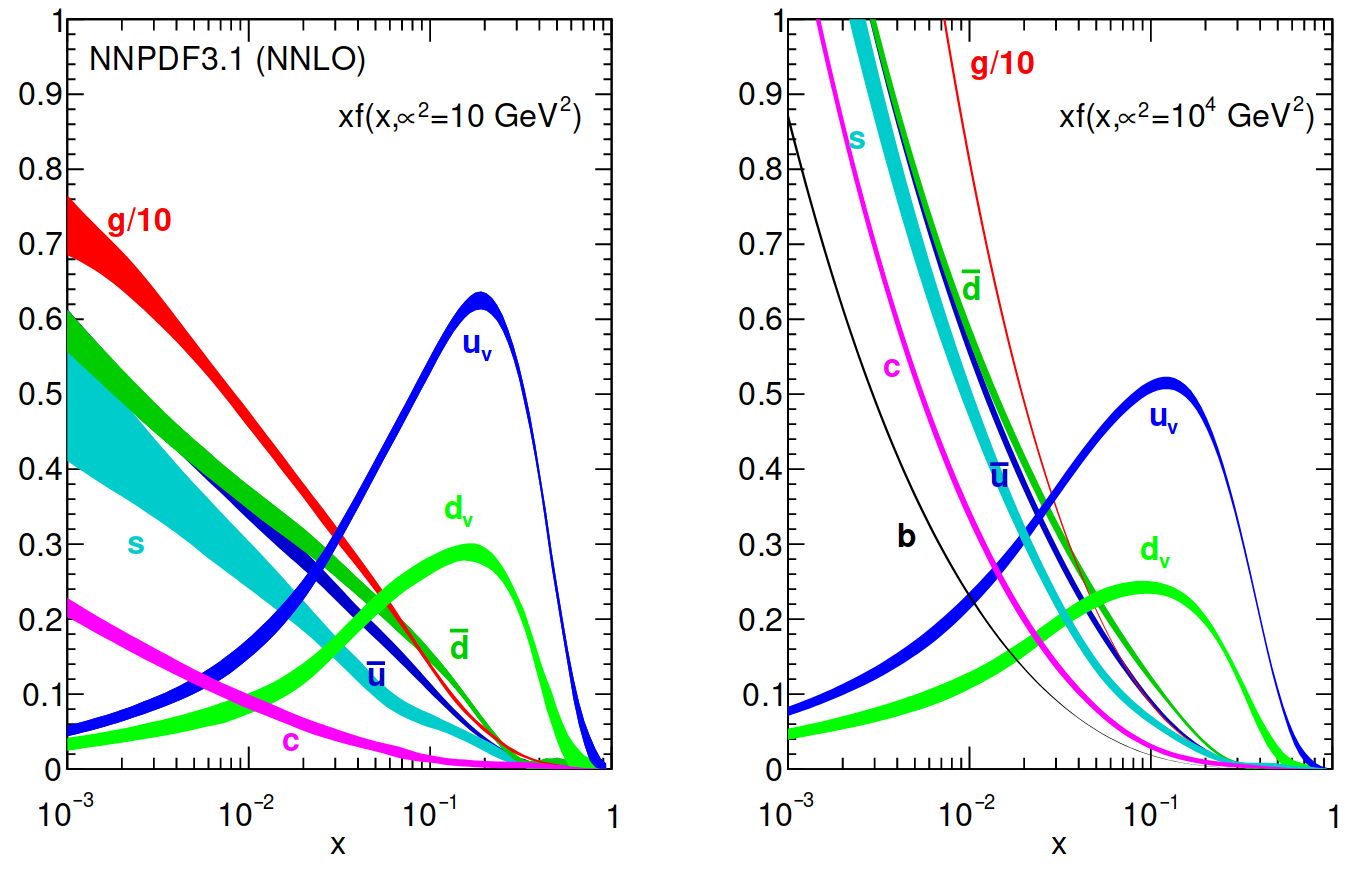
\includegraphics[width=0.7\textwidth]{./figures/theory/nnpdf.png}
    \caption{PDFs for different partons as a function of the Bjorken scaling variable $x$
             for two different factorization scales $Q^2 = \SI{10}{\GeV\squared}$ and $Q^2 = \SI{e4}{\GeV\squared}$.
             The PDF set is NNPDF3.1 (NNLO)~\cite{nnpdf3.1}.}\label{fig:theory:pdfs}
\end{figure}
Another property of quark partons is indicated: It is less probable to find a quark with a higher mass.
The probability to find a photon is highly repressed, in contrast to the gluon PDF, which has the highest value for small $x$.

A dependency on the factorization scale $Q^2$ is recognizable.
The predicted independence of the PDFs from $Q^2$ only holds approximately for certain values.
But the parton model of Feynman still can be used as a foundation to describe inelastic scattering.
There are more complicated models like the \emph{QCD-improved parton model}~\cite{col98}, where
partons are allowed to interact between each other by exchanging gluons.

\todo{Shorten/rephrase section}

\section{The Higgs Boson}\label{sec:theory:higgs}

\subsection{Higgs Boson Production in Proton--Proton Collisions}
\label{sub:theory:higgs:production}

In proton--proton collisions at the LHC the parton model as described above can be applied.
To calculate the cross-section of the production of a particle $X$ in proton--proton collisions the
cross-section at parton level $\hat{\sigma}_{ij\to X}$ has to be weighted with the PDFs and all
possible momentum fractions need to be considered, as prescribed by the factorization theorem~\cite{DRELL1971578}.
Mathematically speaking this is a convolution of the PDFs with the partonic cross-section,
\begin{equation}
    \sigma_{ij\to X} = \int_{0}^{1} \dif x_i \int_{0}^{1} \dif x_j \,
    f_i \left( x_i \right ) f_j \left( x_j \right ) \hat{\sigma}_{ij\to X} \,.
\end{equation}
The general expression of the partonic cross-section is~\cite{Griffiths}
\begin{equation}
    \hat{\sigma}_{ij\to X} = \frac{1}{j} \int \matrixm \left(ij \to X \right) \dif \Phi \,,
\end{equation}
with the matrix element $\matrixm$ which describes the transition probability of the initial state $ij$ to the final state $X$, the
particle flux $j$, and the phase-space factor $\dif \Phi$ depending on the kinematics of the collision.
\\[\baselineskip]
The Higgs boson can be produced in multiple ways, which vary in cross-section and phenomenology.
In \cref{fig:theory:higgs:production} the leading order (LO) Feynman diagrams are shown for the dominant production modes
at the LHC\@.

\todo{Add border to feynman graphs, fix label position}

\begin{figure}[htb]
    \centering
    \begin{subfigure}[t]{0.302\textwidth}
        \includegraphics[width=\textwidth]{feynman/h_ggf.pdf}
        \caption{gluon--gluon fusion}\label{fig:theory:higgs:ggf}
    \end{subfigure}
    \begin{subfigure}[t]{0.201\textwidth}
        \captionsetup{justification=raggedright}
        \includegraphics[width=\textwidth]{feynman/h_vbf.pdf}
        \caption{vector boson fusion}\label{fig:theory:higgs:vbf}
    \end{subfigure}
    \begin{subfigure}[t]{0.201\textwidth}
        \includegraphics[width=\textwidth]{feynman/h_strahl.pdf}
        \caption{Higgs-Strahlung}\label{fig:theory:higgs:vh}
    \end{subfigure}
    \begin{subfigure}[t]{0.246\textwidth}
        \captionsetup{justification=raggedright}
        \includegraphics[width=\textwidth]{feynman/h_top.pdf}
        \caption{associated \mbox{production} with top-quarks}\label{fig:theory:higgs:tassoc}
    \end{subfigure}
    \caption{Feynman diagrams of the dominant production modes of the Higgs boson at the LHC\@. The cross-section
             decreases from left to right.}\label{fig:theory:higgs:production}
\end{figure}

The production mode with the highest cross-section is gluon--gluon fusion (ggF).
This is due to the high contribution of gluon PDF in protons for small momentum fractions $x$, which enables
a quark loop producing a Higgs boson. Because coupling strength of the Higgs boson is proportional to the mass of the
interaction particle, top and bottom quarks contributions dominate in the quark loop.
At leading order only the Higgs boson is produced, therefore it has no transverse momentum.
However, at higher orders final state QCD radiation is possible, which acts as a recoil partner for the Higgs boson.
This is important for measurements, because otherwise the Higgs boson could not be detected.

One order below the cross-section of gluon--gluon fusion the vector-boson fusion (VBF) production mode can be found.
Here two initial state quarks radiate a $Z^0$ or $W^\pm$ boson.
The bosons annihilate and produce a Higgs boson.
The two final state quarks provide a characteristic signature, which is defined by a high mass of the dijet system
and a large separation of the two jets in the pseudorapidity $\eta$ as defined in \cref{eq:pseudorapidity}.

Another production mode is the so-called Higgs-Strahlung, where one weak boson created by the annihilation of
a quark--antiquark pair radiates a Higgs boson.

The Higgs boson production associated with a top-quark pair has a suppressed cross-section compared with the
other production modes.
Because of the large mass of the top quark a high invariant mass is required, which reduces the available phase space.

A distribution of the cross-sections for different Higgs-boson production-modes as a function of the center-of-mass
energy $\sqrt{s}$ is shown in \cref{fig:theory:higgs:xsecs}.
The values of the cross-sections of the most dominant production modes of the Higgs boson at $\sqrt{s} = \SI{13}{\GeV}$
and corresponding uncertainties are listed in \cref{tab:theory:higgs:prodxsec}.

\begin{figure}[htb]
    \centering
    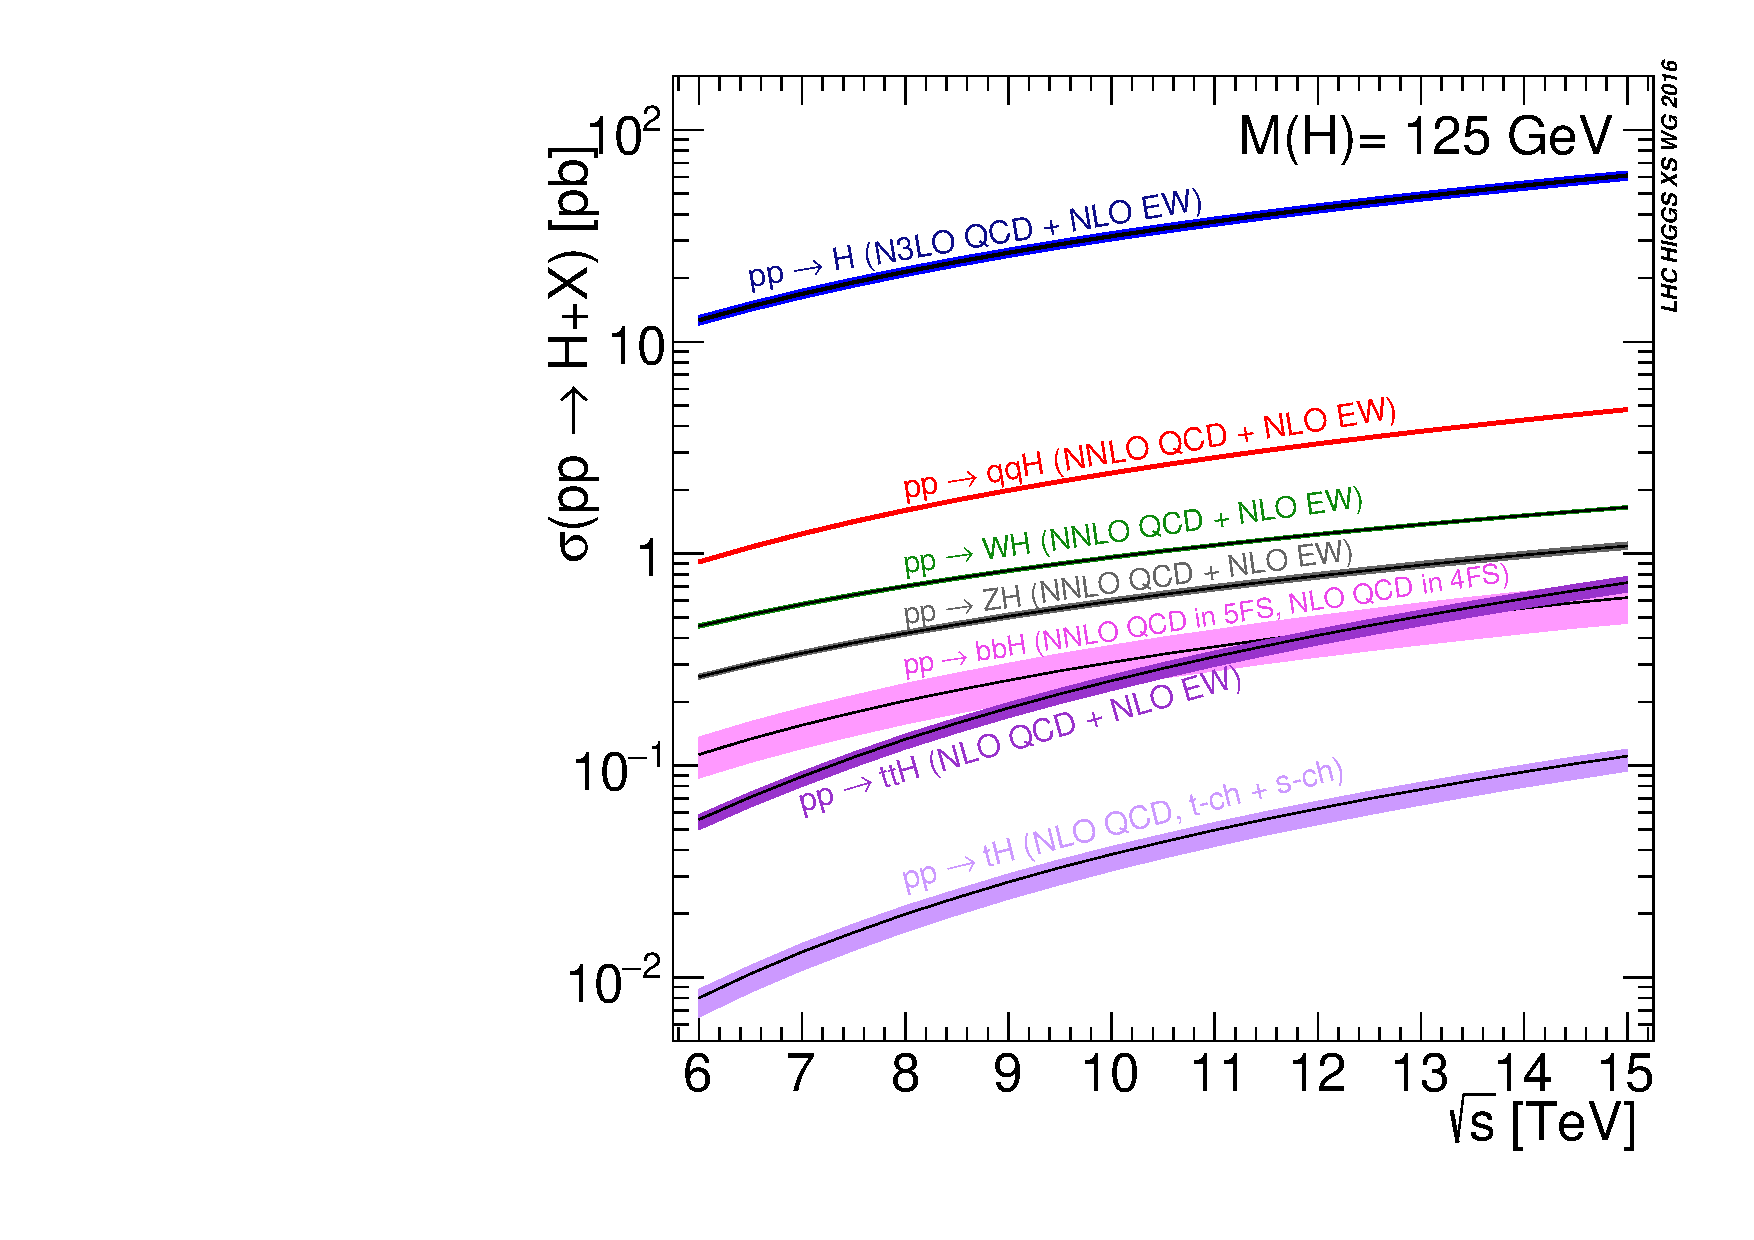
\includegraphics[width=0.45\textwidth]{./figures/theory/higgs_xsec_production.pdf}
    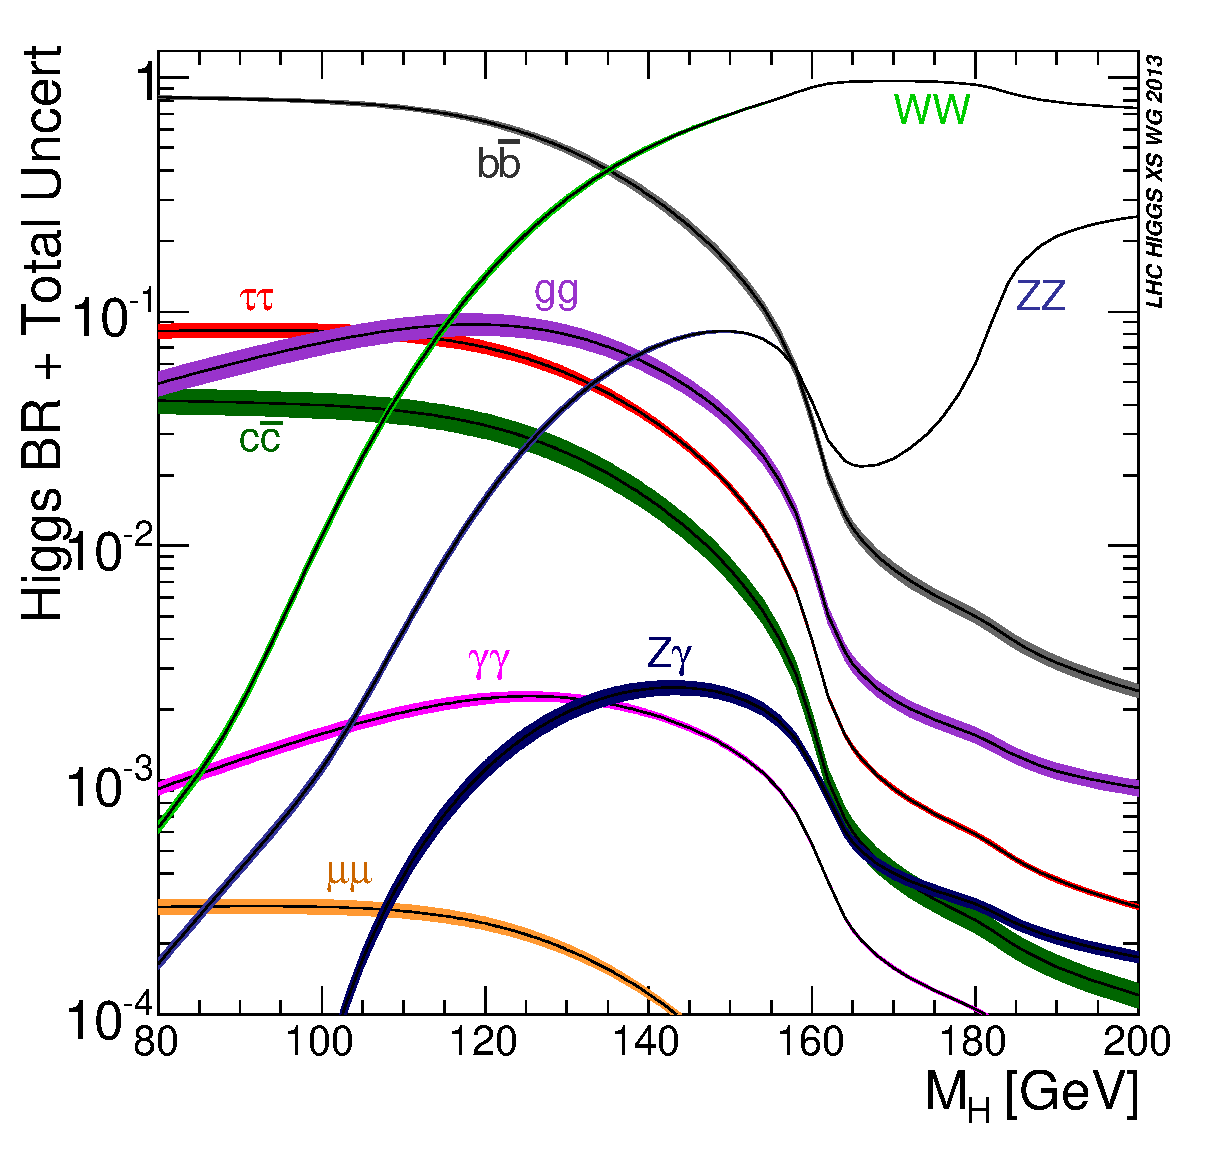
\includegraphics[width=0.45\textwidth]{./figures/theory/higgs_xsec_decay.eps}
    \caption{Production cross-sections of the Higgs boson as a function of the center-of-mass energy $\sqrt{s}$ (left)~\cite{YR4}
             and cross-sections of the Higgs boson decay-modes depeding in the mass $m_H$ of the Higgs boson (right)~\cite{YR3}.}\label{fig:theory:higgs:xsecs}
\end{figure}

\begin{table}[htpb]
    \centering
    \caption{Inclusive cross-sections of different production modes of the Higgs boson with different uncertainties
             for proton--proton collisions at $\sqrt{s} = \SI{13}{\GeV}$ and a mass of the Higgs boson
             of $m_H = \SI{125}{\GeV}$~\cite{YR4}.}\label{tab:theory:higgs:prodxsec}
    \begin{tabular}{cScSS}
        \toprule
        Mode & $\sigma / \si{\pico\barn}$ & $\delta_\text{QCD scale}$ & $\delta_\text{PDF}$ & $\delta_{\alpha_s}$ \\ \midrule
        ggF & 48.58 & \errud{\SI{4.6}{\percent}}{\SI{6.7}{\percent}} & \SI{\pm 1.9}{\percent} & \SI{\pm 2.6}{\percent} \\ \addlinespace[0.2em]
        VBF & 3.782 & \errud{\SI{0.4}{\percent}}{\SI{0.3}{\percent}} & \SI{\pm 2.1}{\percent} & \SI{\pm 0.5}{\percent} \\ \addlinespace[0.2em]
        WH  & 1.373 & \errud{\SI{0.5}{\percent}}{\SI{0.7}{\percent}} & \SI{\pm 1.7}{\percent} & \SI{\pm 0.9}{\percent} \\ \addlinespace[0.2em]
        ZH  & 0.8839 & \errud{\SI{3.8}{\percent}}{\SI{3.1}{\percent}} & \SI{\pm 1.3}{\percent} & \SI{\pm 0.9}{\percent} \\ \addlinespace[0.2em]
        ttH & 0.5071 & \errud{\SI{5.8}{\percent}}{\SI{9.2}{\percent}} & \SI{\pm 3.0}{\percent} & \SI{\pm 2.0}{\percent} \\
        \bottomrule
    \end{tabular}
\end{table}

\subsection{Decay Modes of the Higgs Boson}
\label{sub:theory:higgs:decay}

\section{Measurements of the Higgs Boson at the LHC}
\label{sec:theory:measurements}


